\subsection{Vue d'ensemble et système de coordonnées}\label{chapter-LHC-section-CMS-subsec-overview_and_coordinates}
Le détecteur CMS est installé dans la caverne du point d'interaction numéro~5 du LHC, visible sur la figure~\ref{fig-CERN_map} au Nord de l'installation, dans la commune de Cessy, en France.
Il a été pensé avec pour but premier l'étude de la brisure de symétrie électrofaible et la recherche du boson de Higgs~\cite{cms_letter_intent}.
Pour cela, la conception du détecteur repose sur:
\begin{itemize}
\item un système de détection des muons de haute performance;
\item le meilleur calorimètre électromagnétique possible compatible avec le point précédent;
\item un système de trajectographie central entièrement basé sur des détecteurs au silicium;
\item un calorimètre hadronique avec une résolution suffisante et une bonne herméticité.
\end{itemize}
Son design généraliste permet de nombreuses autres analyses de physique, comme des mesures de précision, la recherche d'une nouvelle physique ou encore les collisions d'ions lourds.
\begin{figure}[b]
\centering
\includegraphics[width=\textwidth]{\PhDthesisdir/plots_and_images/CMS_slices/from_CMS_document_13631-v4/cms_160312_06-FR.tex}
\caption[Vue ouverte du détecteur CMS.]{Vue ouverte du détecteur CMS~\cite{CMS_document_13631-v4}.}
\label{fig-chapter-LHC-section-CMS-subsec-overview_and_coordinates-vue_eclatee_CMS}
\end{figure}
\par La figure~\ref{fig-chapter-LHC-section-CMS-subsec-overview_and_coordinates-vue_eclatee_CMS} présente une vue ouverte du détecteur CMS.
Il possède une forme cylindrique de \SI{28.7}{\meter} de long et \SI{15}{\meter} de diamètre pour un poids total de \num{14000} tonnes.
Il est structuré en couches concentriques, chacune ayant un rôle spécifique détaillé dans les sections qui suivent.
À partir du centre du détecteur, lieu des collisions, se trouvent dans l'ordre
le trajectographe~\cite{CERN-LHCC-98-006},
le calorimètre électronique~\cite{CERN-LHCC-97-033},
le calorimètre hadronique~\cite{CERN-LHCC-97-031},
le solénoïde~\cite{CERN-LHCC-97-010} donnant son \og S \fg{} à CMS et
les chambres à muons~\cite{CERN-LHCC-97-032} donnant son \og M \fg{} à CMS, encastrées dans la culasse d'acier.
Des calorimètres \og \CMSforwards \fg{} se trouvent aux extrémité du détecteur, le long de l'axe du faisceau.
Le détecteur propose ainsi une couverture d'un angle solide de presque $4\pi\usp\SI{}{\steradian}$, \ie\ de presque toutes les directions, ce qui est capital afin de reconstruire les collisions.
\par Le détecteur peut de plus être divisé en trois grandes parties de par sa forme cylindrique.
La première, centrale, est le \og \CMSbarrel \fg, dans laquelle les sous-parties ont une géométrie cylindrique.
Les parties sensibles du détecteur y sont orientées vers l'axe du faisceau.
Aux deux extrémités du détecteur se trouvent les \og \CMSendcaps \fg, dont l'orientation des parties sensibles du détecteur se fait dans le plan transverse au faisceau.
Ces orientations différentes sont bien visibles sur la figure~\ref{fig-chapter-LHC-section-CMS-subsec-overview_and_coordinates-vue_eclatee_CMS}.
\par L'acronyme CMS signifie \emph{Compact Muon Solenoïd}, \ie\ Solénoïde Compact à Muons.
La structure du détecteur, conçue à partir de celle du solénoïde, mène en effet à un design compact pour le système à muons (chambres à muons et culasse d'acier), d'où le qualificatif~\cite{cms_letter_intent}.
\par La géométrie cylindrique du détecteur pousse à définir un système de coordonnées également cylindriques en complément d'un repère cartésien.
Le schéma de la figure~\ref{fig-chapter-LHC-section-CMS-subsec-overview_and_coordinates-CMS_3D_phi_theta_defs} illustre la définition de ces systèmes de coordonnées.
L'origine $O$ des repères est le centre du détecteur où les protons entrent en collision.
Le vecteur de base $\bvec_x$ pointe vers le centre du LHC,
$\bvec_y$ vers le haut ($\vec{g}\cdot\bvec_y<0$) et
$\bvec_z$ est colinéaire au tube de faisceau.
Le trièdre $(\bvec_x, \bvec_y, \bvec_z)$ est direct.
Le plan \plane{x}{y} est nommé \og plan transverse \fg, il est orthogonal aux faisceaux.
Le système de coordonnées cylindriques est défini par la distance à l'origine et deux angles $\theta\in[0,\pi]$ et $\phi\in[-\pi,\pi]$.
L'angle entre le vecteur $\vec{a}$ à caractériser et $\bvec_z$ est $\theta$.
L'angle entre $\vec{a}$ et $\bvec_x$ dans le plan transverse est $\phi$.
\begin{figure}[h]
\centering
{\tdplotsetmaincoords{70}{115}
\tdplotsetrotatedcoords{-90}{-90}{-90}
\begin{tikzpicture}[tdplot_rotated_coords,scale=1.25]
%% base
\draw [->] (0,0,-3)--(0,0,3) node[above] {$\bvec_z$};
\draw [->] (0,0,0)--(1,0,0) node[above] {$\bvec_x$};
\draw [->] (0,0,0)--(0,1,0) node[above] {$\bvec_y$};

%% CMS barrel
\draw (0,0,-2.1) circle (1.5);
\draw (0,0,2.1) circle (1.5);
\def\CMSphiangle{70}
\draw ({1.5*cos(\CMSphiangle)},{1.5*sin(\CMSphiangle)},-2.1) --+(0,0,4.2);
\draw ({1.5*cos(180+\CMSphiangle)},{1.5*sin(180+\CMSphiangle)},-2.1) --+(0,0,4.2);

%% beam
%\draw [ltcolorred, very thick, -latex] (0,0,-2)--(0,0,0);
%\draw [ltcolorred, very thick, -latex] (0,0,2)--(0,0,0);
%% particule sortante
\draw [ltcolorblue, thick, -latex] (0,0,0)--(1.5,1.5,{1.5*2^0.5}) node [right] {$\vec{a}$};
%% vertex primaire
%\fill [ltcolororange] (0,0,0) circle (2pt);

%% track plane
\def\CMSphiangle{45}
\draw [densely dotted] ({1.5*cos(\CMSphiangle)},{1.5*sin(\CMSphiangle)},-2.1) -- ({1.5*cos(\CMSphiangle)},{1.5*sin(\CMSphiangle)},2.1) -- ({-1.5*cos(\CMSphiangle)},{-1.5*sin(\CMSphiangle)},2.1) -- ({-1.5*cos(\CMSphiangle)},{-1.5*sin(\CMSphiangle)},-2.1) --({1.5*cos(\CMSphiangle)},{1.5*sin(\CMSphiangle)},-2.1);

%% phi angle
\draw [densely dotted] (0,0,2.1)--(1.5,0,2.1);
\draw [-latex] (1,0,2.1) arc (0:45:1);
\draw (.75,.25,2.1) node {$\phi$};

%% theta angle
\tdplotsetrotatedcoords{0}{45}{90}
%\draw [tdplot_rotated_coords, ltcolorgreen,<->] (-2.1,1.5,0)--(2.1,-1.5,0);
%\draw [tdplot_rotated_coords, ltcolorgreen,<->] (-2.1,-1.5,0)--(2.1,1.5,0);
%\draw [tdplot_rotated_coords, ltcolorcyan,<->] (-1.5,2.1,0)--(1.5,-2.1,0);
%\draw [tdplot_rotated_coords, ltcolorcyan,<->] (-1.5,-2.1,0)--(1.5,2.1,0);
\draw [tdplot_rotated_coords,-latex] (1,0,0) arc (0:45:1);
\draw [tdplot_rotated_coords] (22.5:1.2) node {$\theta$};

%% origin
\fill (0,0,0) circle (2pt);
\draw (0,0,0) node [below left] {$O$};
\end{tikzpicture}}
\caption[Système de coordonnées du détecteur CMS.]{Système de coordonnées du détecteur CMS.
Le vecteur de base $\bvec_x$ pointe vers le centre du LHC,
$\bvec_y$ vers le haut ($\vec{g}\cdot\bvec_y<0$) et
$\bvec_z$ est colinéaire au tube de faisceau.
Le trièdre $(\bvec_x, \bvec_y, \bvec_z)$ est direct.
L'angle entre le vecteur $\vec{a}$ à caractériser et $\bvec_z$ est $\theta$.
L'angle entre $\vec{a}$ et $\bvec_x$ dans le plan transverse est $\phi$.}
\label{fig-chapter-LHC-section-CMS-subsec-overview_and_coordinates-CMS_3D_phi_theta_defs}
\end{figure}
\par L'angle $\theta$ n'est généralement pas utilisé directement et est remplacé par la \og pseudo-rapidité \fg{} $\eta$ définie comme
\begin{equation}
\eta = - \ln(\tan(\frac{\theta}{2}))
\mend
\label{eq-chapter-LHC-section-CMS-subsec-overview_and_coordinates-eta_definition}
\end{equation}
La pseudo-rapidité est ainsi égale à zéro dans le plan transverse, \ie\ le plan \plane{x}{y}.
L'usage de cette variable est motivé par la densité de production de particules qui est constante suivant $\eta$ et non selon $\theta$.
De plus, dans la limite \og ultra-relativiste \fg{} \ie\ $\abs{\vec{p}}\gg m$, condition remplie au LHC, la pseudo-rapidité tend vers la rapidité $y$ (à ne pas confondre avec la coordonnée $y$) des particules,
\begin{equation}
y = \frac{1}{2} \ln(\frac{E+p_zc}{E-p_zc})
\mend
\end{equation}
Or la rapidité est un invariant de Lorentz, ainsi au LHC $\eta$ est en très bonne approximation un invariant de Lorentz, contrairement à $\theta$.
La figure~\ref{fig-chapter-LHC-section-CMS-subsec-overview_and_coordinates-CMS-eta-ranges} présente un quadrant du détecteur CMS sur lequel figurent quelques valeurs de pseudo-rapidité et les directions correspondantes dans le plan \plane{y}{z}.
\begin{figure}[h]
\centering
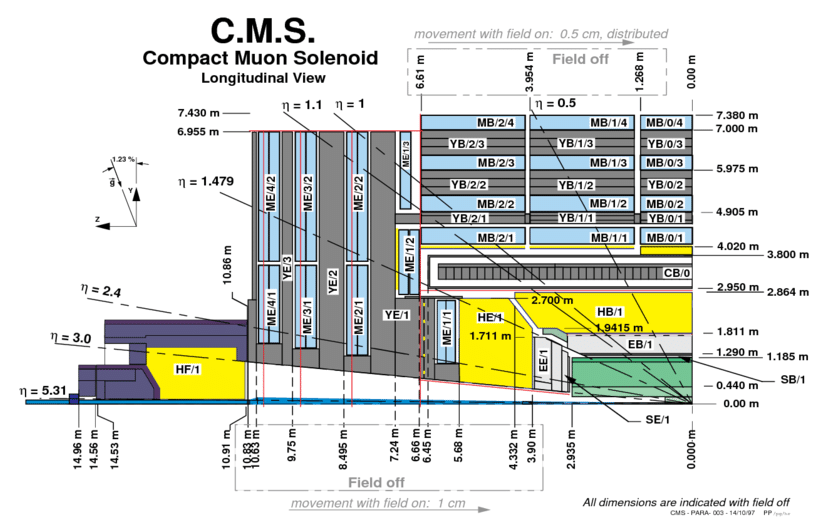
\includegraphics[width=.8\textwidth]{\PhDthesisdir/plots_and_images/from_CMS_alignment_photodetectors/CMS-eta-ranges.png}
\caption[Vue longitudinale d'un quadrant du détecteur CMS.]{Vue longitudinale d'un quadrant du détecteur CMS~\cite{CMS_alignment_photodetectors}. Les directions correspondant à quelques valeurs de pseudo-rapidité sont illustrées et des mesures de distances par rapport au centre du détecteur, lieu des collisions, sont indiquées. Le sol de la caverne présente une inclinaison de \SI{1.23}{\%} par rapport à la direction de la gravité locale $\vec{g}$, ce que montre le schéma à gauche.}
\label{fig-chapter-LHC-section-CMS-subsec-overview_and_coordinates-CMS-eta-ranges}
\end{figure}
\par Du fait de la structure des protons discutée dans la section~\ref{chapter-LHC-section-LHC-subsec-pp_collisions}, lors de la collision, l'impulsion totale selon l'axe des faisceaux est inconnue.
Seule l'impulsion totale dans le plan transverse, \ie\ le plan \plane{x}{y}, est nulle.
C'est pourquoi des variables relatives au plan transverse sont définies, en particulier l'impulsion transverse \vpT, sa norme \pT\ et l'\og énergie transverse \fg{} \ET,
\begin{equation}
\vpT = p_x\bvec_x + p_y\bvec_y
\msep
\pT = \sqrt{p_x^2+p_y^2}
\msep
\ET = E\sin\theta = \frac{E}{\cosh\eta}
\mend
\end{equation}